
\documentclass[a4paper,10pt,fleqn, twocolumn]{IEEETran}
\usepackage{amsfonts}
\usepackage{amsthm}
\usepackage{graphicx}
\usepackage{fancyhdr}



\setlength{\parindent}{3em} \setlength{\oddsidemargin}{0in}
\setlength{\textwidth}{6.5in} % sets 1in left and right margins
\setlength{\topmargin}{0.20in} % change to 0.2in for regular latex
%\setlength{\headheight}{0in}
%\setlength{\footheight}{0.5in}
\setlength{\footskip}{0.5in}
\setlength{\textheight}{9.0in} %sets 1in top and bottom margins
\renewcommand{\baselinestretch}{1} %set to 1.5 for double spacing.



\newcommand{\br}{{\mathbf r}}
\newcommand{\bA}{{\mathbf A}}
\newcommand{\ba}{{\bf a}}
\newcommand{\bb}{{\bf b}}
\newcommand{\bc}{{\bf c}}
\newcommand{\bC}{{\bf C}}
\newcommand{\bg}{{\bf g}}
\newcommand{\bG}{{\bf G}}
\newcommand{\bd}{{\bf d}}
\newcommand{\be}{{\bf e}}
\newcommand{\bs}{{\bf s}}
\newcommand{\bm}{{\bf m}}
\newcommand{\bn}{{\bf n}}
\newcommand{\bu}{{\bf u}}
\newcommand{\bv}{{\bf v}}
\newcommand{\bw}{{\bf w}}
\newcommand{\bx}{{\bf x}}
\newcommand{\by}{{\bf y}}
\newcommand{\bbf}{{\bf f}}
\newcommand{\bE}{{\bf E}}
\newcommand{\bF}{{\bf F}}
\newcommand{\bL}{{\bf L}}
\newcommand{\bM}{{\bf M}}
\newcommand{\bN}{{\bf N}}
\newcommand{\bS}{{\bf S}}
\newcommand{\bT}{{\bf T}}
\newcommand{\bD}{{\bf D}}
\newcommand{\bX}{{\bf X}}
\newcommand{\bP}{{\bf P}}
\newcommand{\bQ}{{\bf Q}}
\newcommand{\bI}{{\bf I}}
\newcommand{\bR}{{\bf R}}
\newcommand{\bU}{{\bf U}}
\newcommand{\bV}{{\bf V}}
\newcommand{\bW}{{\bf W}}
\newcommand{\bJ}{{\bf J}}
\newcommand{\bB}{{\bf B}}
\newcommand{\bzero}{{\bf 0}}
\newcommand{\bgamma}{{\mbox {\boldmath $\gamma$}}}
\newcommand{\btheta}{{\mbox {\boldmath $\theta$}}}
\newcommand{\bLambda}{{\mbox {\boldmath $\Lambda$}}}
\newcommand{\bPsi}{{\mbox {\boldmath $\Psi$}}}
\newcommand{\bPhi}{{\mbox {\boldmath $\Phi$}}}
\newcommand{\bcA}{{\mbox {\boldmath ${\cal A}$}}}
\newcommand{\bcB}{{\mbox {\boldmath ${\cal B}$}}}
\newcommand{\bcC}{{\mbox {\boldmath ${\cal C}$}}}
\newcommand{\bcD}{{\mbox {\boldmath ${\cal D}$}}}
\newcommand{\bcF}{{\mbox {\boldmath ${\cal F}$}}}
\newcommand{\bcN}{{\mbox {\boldmath ${\cal N}$}}}
\newcommand{\bcS}{{\mbox {\boldmath ${\cal S}$}}}
\newcommand{\bcH}{{\mbox {\boldmath ${\cal H}$}}}
\newcommand{\bcI}{{\mbox {\boldmath ${\cal I}$}}}
\newcommand{\bcR}{{\mbox {\boldmath ${\cal R}$}}}

\title{Blind Adaptive Multiuser Detection}
\author{Shu Wang, Sang G. Kim, Byung K. Yi, Li-Hsiang Sun, Ki Y. Kim,
\\Su K. Lee and Hobin Kim \\ LGE Mobile Research
Center\\San Diego, CA 92131}
\date{}
\begin{document}
\maketitle
\begin{abstract}\small
In this paper, a new blind multiuser detection model and framework
are proposed. Based on this blind detection framework, several
novel blind multiuser detection algorithms are developed using
least-squares-based (LS) estimations, including LS estimation,
total least-squares (TLS) estimation and mixed LS/TLS (MLS)
estimation, best least unbiased (BLU) estimation, minimum
mean-square error (MMSE) estimation criteria. All proposed
algorithms are simple and direct. Only the spreading sequence and
timing of the desired user(s) are involved. No prior knowledge or
estimation of other unknown users is required. They can be easily
extended to CDMA reverse links too. Theoretical analysis and
computer simulations are finally provided to demonstrate the
proposed schemes.
\end{abstract}

\section{Introduction}
Multiuser detection strategy is a method for mitigating MAI
effects with exploiting interference structure. It has been
extensively investigated over the past decade since MAI is the
dominant impairment for CDMA systems and even exists in perfect
power-controlled CDMA systems~\cite{Verd98}. Recent research has
been devoted to blind multiuser detection and subspace-based
signature waveform estimation schemes for achieving better
performance and higher
capacity~\cite{Madh94,Honi95,Poor97,Wang98,Torl97,Liu96}. Blind
multiuser detectors can achieve good performance with only the
knowledge of the timing and signature waveform of desired user(s)
while they don't require intensive computation, compared with
optimal multiuser detectors and some conventional multiuser
detectors. The assumption for blind detection design obviously is
much closer to practical applications.


There are two popular approaches for designing blind multiuser
detectors. One is to use statistical optimization criteria, e.g.
MMSE~\cite{Madh94,Honi95}, for blind multiuser detection. The
other approach is to estimate and restore the conventional system
model and therefore use conventional multiuser detection
techniques. Many subspace-based approaches are the examples using
this approach~\cite{Wang98,Yang95,Wang99}. In this paper, we
proposed an alternative approach for forward-link blind multiuser
receiver design with extending the semiblind approach
in~\cite{Wang03d,Wang03e}. Instead of using the conventional
multiuser system model, a new blind multiuser system model is
constructed for each individual receiver. Different from the
conventional model including all users' amplitude and spreading
sequence information, the proposed blind model only requires
desired users' spreading sequences and several previous received
signal vectors. Instead of the original spreading sequence matrix,
a blind spreading sequence matrix, which is different for
different users and can even change from time to time, is used in
the blind model. Based on this blind system model, a blind
multiuser detection framework and therefore several blind
multiuser detectors using LS-based estimations, BLU estimation and
MMSE estimation are proposed. In the present multiuser blind
detectors, only the signature and timing of the desired user are
utilized. These algorithms are simple and direct. No search
procedure is employed as many other semi-blind/blind
detectors~\cite{Torl97,Wang98}. Theoretical analysis and computer
simulations are finally presented to demonstrate the performance
of these blind detectors.

\section{System Model And Problem Description}
We consider forward-link transmissions in a single-cell DS/CDMA
system. There are $K$ active users over the multipath channel with
$P$ strong paths~\footnote{Strong paths are those paths which will
be explicitly combined by RAKE receiver.} and the channel is an
additive white Gaussian noise (AWGN) channel. The baseband
representation of the received signal due to user $k$ is given by
\begin{equation}
\begin{array}{rcl}
r_k(t)&=&\sum\limits_{p=1}^{P}\alpha_{pk}A_k[n]
b_k[n]c_k(t-nT-\tau_p)
\end{array}
\end{equation}
\noindent where $\alpha_{pk}$ is the $p$th path loss of user $k$'s
signal, $b_k{[n]}$ is the $n$th bit sent by user $k$. We assume
that the $\left\{b_k{[n]}\right\}$ are independent and identically
distributed random variables with $E\left\{b_k{[i]}\right\}=0$ and
$E\left\{|b_k{[i]}|^2\right\}=1$. The parameters $c_k(t)$ denote
the normalized spreading signal waveform of user $k$ during the
interval $[0,\ T]$, $\tau_1\leq\tau_2\leq\ldots\leq\tau_P$,
denotes $P$ different transmission delays from the base station to
user $k$ and $A_k[n]$ is the amplitude of the received signal for
user $k$ at time $t=n$. The total baseband signal received by user
$k$ is
\begin{equation}
\begin{array}{rcl}
\tilde{r}(t)&=&\sum\limits_{k=1}^{K}r_k(t)
\end{array}
\end{equation}
The received signal $\tilde{r}(t)$ is passed through the
corresponding chip matched filter (CMF) $\phi(t)$ and RAKE
combiner. The combined output $r(t)$ is~\footnote{Without loss of
the generality, we drop the time index $n$ in the following
discussion.}
\begin{equation}\hspace{-0.0in}
\begin{array}{rcl}
r(t)&=&A_k b_k c_k(t-nT-\tau_1)\otimes \phi(t-\tau_1)+ \\
&&\hspace{0.0in} m_{\rm ISI}(t) + m_{\rm MAI}(t) + n(t)
\end{array}\label{r_t}
\end{equation}
\noindent where
\begin{equation} \hspace{-0.05in}
\begin{array}{rcl}
 m_{\rm ISI}(t)&=&\\
 &&\hspace{-0.83in}\sum\limits^{P}_{p\neq
q}\beta_{qk} \alpha_{pk}A_kb_kc_k(t-nT+\tau_{q1}-\tau_1)\otimes
\phi(t-\tau_1)
\end{array}
\end{equation}
\noindent is the intersymbol interference (ISI) to user $k$,
\begin{equation} \hspace{-0.17in}
\begin{array}{rcl}
m_{\rm MAI}(t)&=&\sum\limits_{i\neq
 k}^{K}A_ib_ic_i(t-nT-\tau_1)\otimes\phi(t-\tau_1)+\\
 &&\hspace{-0.75in}\sum\limits_{i\neq
 k}^{K}\sum\limits^{P}_{p\neq
q}\beta_{qk}
\alpha_{pi}A_ib_ic_i(t-nT+\tau_{q1}-\tau_p)\otimes\phi(t-\tau_1)
\end{array}
\end{equation}
\noindent is the MAI to user $k$, $\beta_{qk}$ is the weight of
the $q$th RAKE finger with
$\sum\limits_{q=1}^{P}\beta_{qk}\alpha_{qk}=1$ and $\tau_{q1} =
\tau_{q}-\tau_1$ is the propagation delay difference between the
$1$st path and $p$th path. $\otimes$ denotes the convolutional
product. $n(t)$ is AWGN with variance $\sigma^2$. The user $k$'s
RAKE output can be sampled at $f_s=1/T_s$ and expressed by
\begin{equation}\hspace{-0.1in}
\begin{array}{rcl}
\br&=&\left[
\matrix{r(nT+T_s+\tau_1)&\ldots&r(nT+LT_s+\tau_1)}\right]^{\rm
T}\\
 &=&\sum\limits_{k=1}^{K} A_k b_k \bs_k + \bn \\
 &=&\bS \bA \bb + \bn
\end{array}\label{r_sync}
\end{equation}
\noindent where $\bS=[\bs_1\ \bs_2\ \ldots\ \bs_K]$ is the
received spreading sequence matrix, whose columns contain possible
ISI and MAI information, and $L=T/T_s$ is the number of samples
per symbol, which should not be less than the spreading gain
$L_c$.

Because of $m_{\rm MAI}(t)$ existing in the received signal
$r(t)$, the performance of conventional matched filter receiver
will suffer from the so-called near-far problem where a strong or
near-by user can prevent the detection of weak or far-away users.
Multiuser detection is the receiver technique for solving the
near-far problem. Linear blind multiuser detector was proposed by
Shnidman~\cite{Shni67}. Compared with other centralized schemes,
linear blind multiuser detector can be implemented in a
decentralized fashion where only the user or users of interest
need be demodulated and therefor is much closed to practical
applications. Most linear multiuser detectors for demodulating the
$k$th user's data bit in (\ref{r_sync}) is in the form of a
correlator followed by a hard limiter, which could be expressed as
\begin{equation}
\begin{array}{rcl}
\hat{b}_k &=& \mbox{sign}\{\bw_k^{\rm T}\br\}
\end{array} \label{linear}
\end{equation}
\noindent where $\bw_k \in \mathbb{R}^{L\times 1}$ is the linear
representation of multiuser detector.

\section{Blind Multiuser Detection Framework\label{BMUD_model}}
\begin{figure} \center{
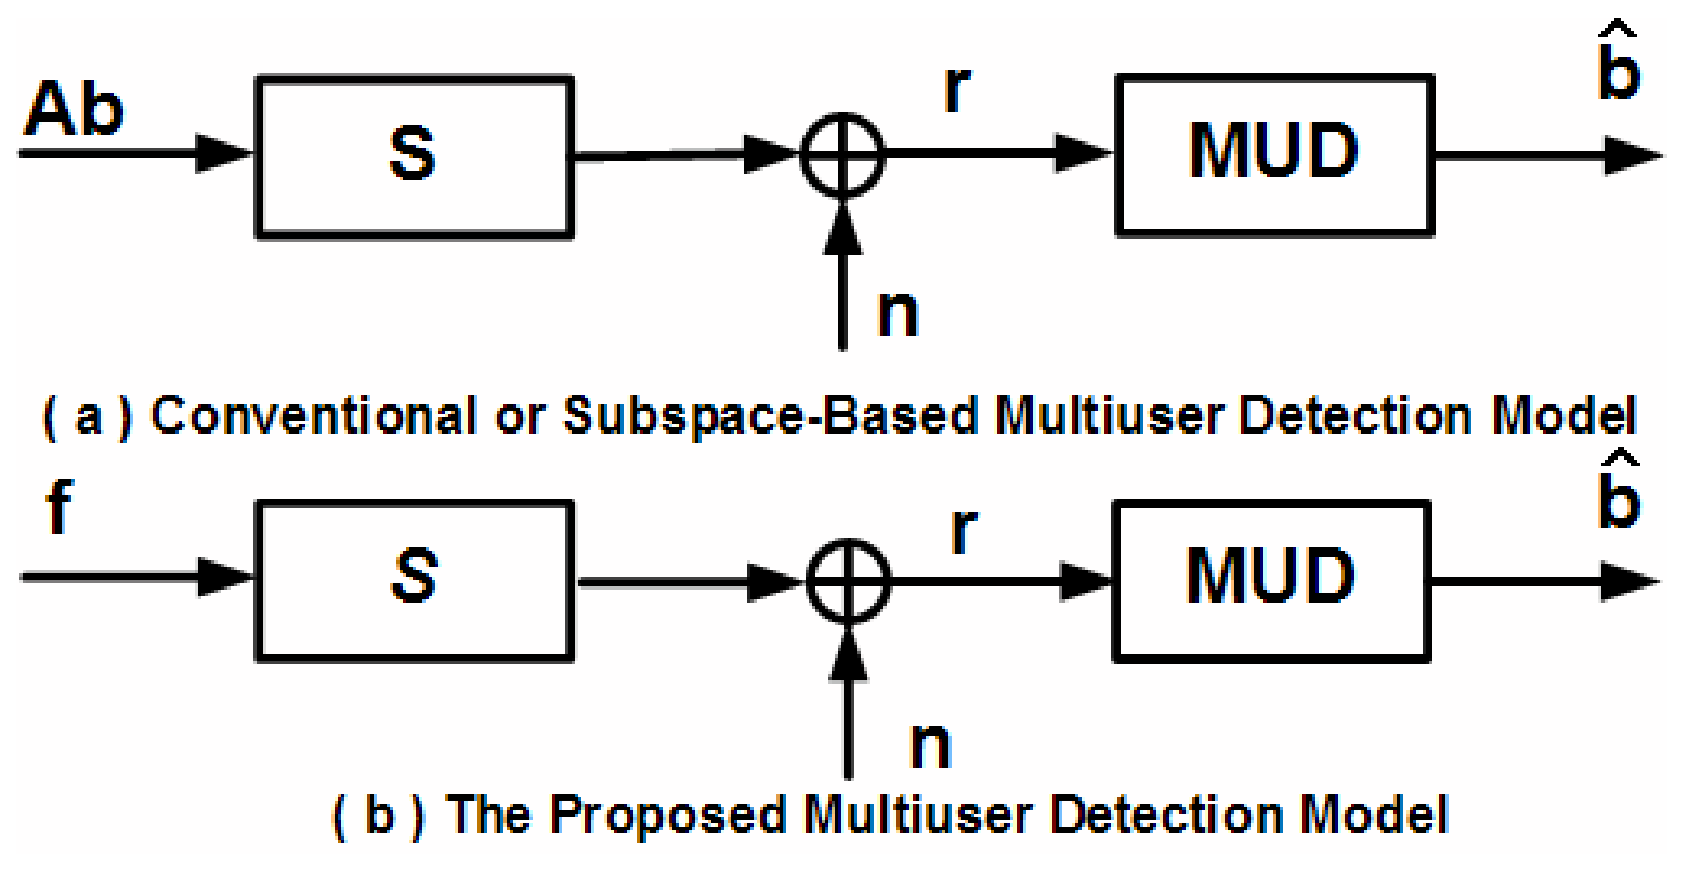
\includegraphics[width=2.8in]{MUD_model.eps}
\caption{Multiuser detection models.  } }\label{MUD_model}
\end{figure}

Differen to most existing multiuser detection algorithms, we take
a different approach for blind multiuser detection. We propose a
new blind multiuser system model using a blind but "faked"
spreading matrix for the desired user(s) which can be shown in
Fig.~\ref{MUD_model}. We say it is a blind but "faked" because 1)
it consists only of several known spreading sequence and also
several previous received signal vectors, 2) it isn't the original
spreading sequence matrix but works like the original one. Without
loss of the generality, only the bits $b_1$ sent by user $1$ in a
synchronous CDMA system are considered and the $L\times M$ blind
spreading sequence matrix $\bcS$ is defined by
\begin{equation}
\begin{array}{rcl}
\bcS&=&[\matrix{\bs_1&\ldots&\bs_G&{\br}_{1}&{\br}_{2}&\ldots&{\br}_{M-G}}]\\
\end{array} \label{S_0}
\end{equation}
\noindent where $\bs_g$, $g=1,\ 2,\ \ldots,\ G$, denote the group
of $G$ spreading waveforms which are already known to user $1$.
${\br}_m$, $m=1,\ 2,\ \ldots,\ M-G$, are $M-G$ previously received
independent signal vectors. The relationship between the proposed
blind spreading matrix $\bcS$ and the original spreading matrix
$\bS$ can be given by
\begin{equation}
\begin{array}{rcl}
\bcS &=&\bS\bB + {\bN}\\
\end{array}
\end{equation}
\noindent where the first $G$ columns of $\bcS$ and $\bS$ are
same,
\begin{equation}\hspace{-0.0in}
\begin{array}{l}
 \bB=\left[\matrix{\bI & \bar\bD\cr\bzero&\tilde\bD }\right]=\left[\matrix{\bE & \matrix{\bar\bD\cr \tilde{\bD}} }\right]
  =\left[\matrix{\bG \cr \matrix{\mathbf{0}& \tilde{\bD}}
 }\right]
\end{array}\label{B}
\end{equation}
\noindent is the $K\times M$ data matrix associated with $\bcS$.
$\bE=[\matrix{\bI&\bzero}]^{\rm T}$, $\bG = \left[\matrix{\bI&
\bar\bD}\right]$ is the $G\times M$ matrix composed by known data
in $\bcS$. $\mbox{rank}\{\tilde{\bD}\}=K-G$ and
$\mbox{rank}\{\bB\}\geq K$. Combining (\ref{r_sync}) and
(\ref{S_0}), the received signal vector $\br$ in (\ref{r_sync})
can now be expressed by
\begin{equation}
\begin{array}{rcl}
\br&=&\bcS\bbf + \bar{\bn} \label{r_blind}
\end{array}
\end{equation}
\noindent where the $M \times 1$ vector $\bbf$ is termed the
detection vector defined by
\begin{equation}
\begin{array}{rcl}
\bbf&=&\bB^{+}\bar\bb
\end{array} \label{DetectorVector}
\end{equation}
\noindent where $[\cdot]^{+} $ denotes the general inverse
operator and $\bar\bb=\bA \bb$. $\bar{\bn}$ is the new $L\times 1$
noise vector defined by
\begin{equation}
\begin{array}{rcl}
\bar{\bn}&=&\bn-{\bN}\bB^{+}\bar\bb
\end{array} \label{new_noise}
\end{equation}
With (\ref{DetectorVector}), the bit $b_1$ sent for user 1 can be
detected using the following equations:
\begin{equation}\hspace{0.2in}
\begin{array}{l}
\hat{\bb}_1
=\left[\matrix{\hat{b}_1&\hat{b}_2&\ldots&\hat{b}_G}\right]^{\rm
T}=\mbox{sgn}\left\{\bG\bbf\right\}\
\end{array}, \label{b_estimation}
\end{equation}
\begin{equation}\hspace{-0.40in}
\begin{array}{l}
\hat{\ba}_1
=\left[\matrix{\hat{A}_1&\hat{A}_2&\ldots&\hat{A}_G}\right]^{\rm
T}=\left|\bG\bbf\right|\ .
\end{array} \label{A_estimation}
\end{equation}
\noindent The detection for user $1$ now becomes how to
efficiently estimate $\bbf$ and initialize/update $\bcS$ or $\bG$.
In the following, we discuss various algorithms for estimating
$\bbf$ and then formulate different blind multiuser detectors. How
to update $\bcS$ will be discussed in Section \ref{updatingG}.


\section{Blind Multiuser Detectors\label{LBD}}
\subsection{Least Squares Detection } At first, we assume that
the measurements of $\bcS$ are assumed to be free of error. All
errors are confined to the received vector $\br$. Hence, the
detection vector can be estimated with solving the following
equation
\begin{equation}
\begin{array}{rcccl}
{\bbf}_{\rm
LS}&=&\matrix{\mbox{arg}\min\limits_{\bx}\left\|\br-\bcS\bx\right\|_2}&=&\bcS^+\br
\end{array}
\label{LSProb}
\end{equation}
\noindent and the bit vector for user $1$ can be detected by
\begin{equation}
\begin{array}{rcl}
\hat{\bb}_1&=&\mbox{sign}\left\{\bG\bcS^{+}\br\right\}
\end{array} \label{w_LS}
\end{equation}

\subsection{Total Least Squares Detection}
It assumes $\bcS$ to be error-free in the previous LS estimation.
This assumption is not entirely accurate according to the
definition in (\ref{S_0}) since there is a noise term $\bN$.
Problem (\ref{LSProb}) can then be transformed into the TLS
problem:
\begin{equation}
\begin{array}{l}
\left[\matrix{\bcS_{\rm TLS}\cr\bbf_{\rm
TLS}}\right]=\matrix{\mbox{arg}\min\limits_{\bar{\bcS},\
\bx}\left\|\left[ \matrix{\bcS\cr\br} \right] - \left[
\matrix{\bar{\bcS}\cr\bar{\bcS}\bx}\right]\right\|_2}
\end{array}.
\label{TLSProb}
\end{equation}
 Let $\bcS=\bU^{'}\mathbf{\Sigma}^{'}\bV^{'\rm T}$ and
$[\bcS\ \br]=\bU\mathbf{\Sigma}\bV^{\rm T}$ be the SVD of $\bcS$
and $[\bcS\ \br]$, respectively. If $\sigma_K^{'}
> \sigma_{K+1}$, TLS estimation of $\bbf$ then is~\cite{Huff91}
\begin{equation}
\bbf_{\rm TLS} = \left(\bcS^{\rm
T}\bcS-\sigma_{K+1}^2\bI\right)^{-1}\bcS^{\rm T}\br
\end{equation}
\noindent and the bit vector for user $1$ can be detected by
\begin{equation}
\begin{array}{rcl}
\hat{\bb}_1&=&\mbox{sign}\left\{\bG(\bcS^{\rm
T}\bcS-\sigma_{K+1}^2\bI)^{-1}\bcS^{\rm T}\br\right\}
\end{array} \label{w_LS}
\end{equation}

\subsection{Mixed LS/TLS Detection}
Though there exists a noise or error matrix $\bN$ in $\bcS$ from
(\ref{S_0}), its first $G$ columns are exactly known to be
noise-free or error-free. Hence, to maximize the estimation
accuracy of the detection vector $\bbf$, it is natural to require
the corresponding columns of $\bcS$ to be unperturbed since they
are known exactly. Problem (\ref{LSProb}) or (\ref{TLSProb}) can
then be transformed into the following MLS problem:
\begin{equation}
\begin{array}{l}
\left[\matrix{\bcS_{\rm MLS}\cr\bbf_{\rm
MLS}}\right]=\matrix{\mbox{arg}\min\limits_{\bar{\bcS},\
\bx}\left\|\left[\matrix{\tilde{\bcS}\cr\br}\right]-\left[\matrix{\bar{\bcS}\cr[\bs_1\
 \bar{\bcS}]\bx}\right]\right\|_{2} }
\end{array}.\label{MLSProb}
\end{equation}
Consider the MLS problem in (\ref{MLSProb}) and perform the
Householder transformation $\bQ$ on the matrix
$[\matrix{\bcS&\br}]$ so that
\begin{equation}\hspace{-0.14in}
\begin{array}{l}
\bQ^{\rm
T}[\matrix{\bs_1&\ldots&\bs_G&\bar{\bcS}&\br}]=\left[\matrix{\bR_{11}&\bR_{12}&\br_{1r}\cr
\mathbf{0}&\bR_{22}&\br_{2r}}\right]
\end{array}
\end{equation}
where $\bR_{11}$ is a $G\times G$ up triangle matrix, $\br_{1r}$
is a $G\times 1$ vector and $\br_{2r}$ is a $(L-G)\times 1$
vector. Denote $\sigma'$ as the smallest singular value of
$\bR_{22}$ and $\sigma$ as the smallest singular value of
$[\matrix{\bR_{22}&\br_{2r}}]$. If $\sigma'>\sigma$, then the MLS
solution uniquely exists and is given by~\cite{Huff91}
\begin{equation}\hspace{-0.09in}
\begin{array}{rcl}
\bbf_{\rm MLS}&=&\left(\bcS^{\rm
T}\bcS-\sigma^2\left[\matrix{\bzero&\mathbf{0}\cr\mathbf{0}&\mathbf{I}_{M-G}}\right]\right)^{-1}\bcS^{\rm
T}\br
\end{array}.
\end{equation}
\noindent and the bit vector for user $1$ can be detected by
\begin{equation}\hspace{-0.2in}
\begin{array}{l}
\hat{\bb}_1=\mbox{sign}\left\{\bG\left(\bcS^{\rm
T}\bcS-\sigma^2\left[\matrix{\bzero&\mathbf{0}\cr\mathbf{0}&\mathbf{I}_{M-G}}\right]\right)^{-1}\bcS^{\rm
T}\br\right\}
\end{array} \label{b_MLS}
\end{equation}

\subsection{Best Linear Unbiased Detection}
We assume the linear structure
\begin{equation}
\begin{array}{rcl}
{\bbf}_{\rm BLU}&=&\bW_{\rm BLU}^{\rm T}\br
\end{array}
\end{equation}
\noindent for this so-called best linear unbiased estimator
(BLUE). Matrix $\bW_{\rm BLU}$ is designed such that: 1) $\bcS$
must be deterministic, 2) $\bar{\bn}$ must be zero mean with
positive definite known covariance matrix $\bC_{\bar{\bn}}$, 3)
${\bbf}_{\rm BLU}$ is an unbiased estimator of $\bbf$, 4) and the
error variance for each of the $M$ parameters is minimized as
\begin{equation}
\begin{array}{rcl}
\bW_{\rm BLU}&=&\min\limits_{\bW_{\bbf}}
\mbox{var}\left\{\bW_{\bbf}^{\rm T}\br\right\}
\end{array}
\end{equation}
\noindent In this way, ${\bbf}_{\rm BLU}$ will be unbiased and
efficient, within the class of linear estimators, by design. The
resulting best linear unbiased estimator is (Gauss-Markov
Theorem):
\begin{equation}
\begin{array}{rcl}
{\bbf}_{\rm BLU}&=&(\bcS^{\rm
T}\bC_{\bar{\bn}}^{-1}\bcS)^{-1}\bcS^{\rm
T}\bC_{\bar{\bn}}^{-1}\br\ .
\end{array} \label{BLUE}
\end{equation}
\noindent The covariance matrix of ${\bbf}_{\rm BLU}$ given by
\begin{equation}
\begin{array}{rcl}
{\bC}_{\bbf_{\rm BLU}}&=&(\bcS^{\rm
T}\bC_{\bar{\bn}}^{-1}\bcS)^{-1}
\end{array}.
\end{equation}
\noindent Though the PDF of $\bB$ may be determined, the PDF of
$\bB^{+}$ is largely unknown. This makes it is hard to calculate
the closed-form solution of $\bC_{\bbf}$ and $\bC_{\tilde{\bn}}$.
However, with Girko's Law, when $\alpha=(K-G)/(M-G)$ is fixed,
$K$, $M$ $\rightarrow\infty$, the diagonal element of
$\frac{1}{M-G}\tilde{\bD}^+\tilde{\bb}\tilde{\bb}^{\rm
T}\tilde{\bD}^{\rm +T}$ may be approximated
by~\cite{Muller,Hanly90}
\begin{equation}
\begin{array}{rcl}
\lim\frac{1}{M-G}\left[\tilde{\bD}^+\tilde{\bb}\tilde{\bb}^{\rm
T}\tilde{\bD}^{\rm +T}\right]_{ii}^{-1}&=&1-\alpha
\end{array}.
\end{equation}
\noindent So, $\bC_{\bbf}$ can be decided by
\begin{equation}
\begin{array}{rcl}
\bC_{\bbf}&=&\left[\matrix{\frac{2M-K-G}{M-K}\bA_1^2&\bzero^{\rm
T}\cr\bzero&\frac{1}{M-K}\bI}\right]
\end{array},
\end{equation}
\noindent where $\bA_1=\mbox{diag}\{\ba_1\}$,
\begin{equation}
\begin{array}{rcl}
\bC_{\bar\bn}&=&\sigma^{2}\frac{2M-K-G}{M-K}\bI
\end{array}\label{noise_var_new}
\end{equation}
\noindent and the bit vector for user $1$ can be detected by
\begin{equation}
\begin{array}{rcl}
\hat{\bb}_1&=&\mbox{sign}\left\{\bG(\bcS^{\rm
T}\bcS)^{-1}\bcS^{\rm T}\br\right\}
\end{array}
\end{equation}

\subsection{Minimum Mean Square Detection}
Now we estimate $\bbf$ based on MMSE criterion. This class of
estimators are generically termed Wiener filter. Given
measurements $\br$, the MSE estimator of $\bbf$, ${\bbf}_{\rm MS}
= f( \br )$, minimizes the mean-squared error $J_{\rm
MSE}=E\{||\bbf-\hat{\bbf}||_2^2\}$. The function $f(\br)$ may be
nonlinear or linear and its exact structure is determined by
minimizing $J_{\rm MSE}$. When $\bbf$ and $\br$ are jointly
Gaussian, the linear estimator $\bW_{\rm MMS}$ that minimizes the
mean-sqared error is (Bayesian Gauss-Markov Theorem)
\begin{equation}
\begin{array}{rcl}
{\bbf}_{\rm MMS}&=&(\bC_{\bbf}^{-1}+\bcS^{\rm
T}\bC_{\bar{\bn}}^{-1}\bcS)^{-1}\bcS^{\rm
T}\bC_{\bar{\bn}}^{-1}\br
\end{array} \label{MSE}
\end{equation}
\noindent and the bit vector for user $1$ can be detected by
\begin{equation}\hspace{-0.05in}
\begin{array}{l}
\hat{\bb}_1=\mbox{sign}\left\{\bG(\bC_{\bbf}^{-1}+\bcS^{\rm
T}\bC_{\bar{\bn}}^{-1}\bcS)^{-1}\bcS^{\rm
T}\bC_{\bar{\bn}}^{-1}\br\right\}
\end{array}
\end{equation}

\section{Blind Adaptive Multiuser Detection\label{updatingG}}
\begin{figure}
\center{
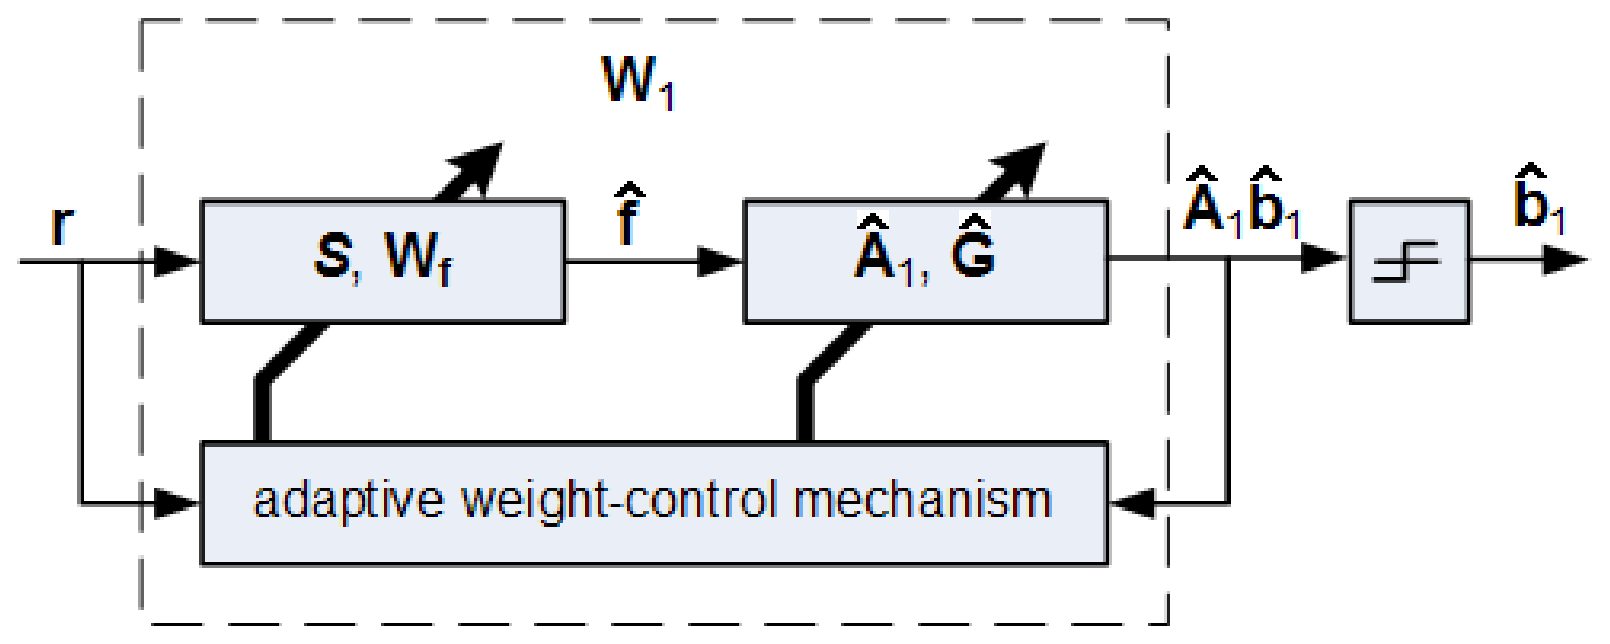
\includegraphics[width=3.1in]{BMUD_structure10.eps}
\caption{ The proposed adaptive blind multiuser detection
structure.} }\label{AMUDstruct}
\end{figure}
In Fig. 2, an adaptive structure of the presented blind multiuser
detection scheme is presented for time-variant channels. Following
the well-known Woodbury matrix inverse lemma~\cite{Golu96}, an
adaptive implementation of  the proposed least-square blind
detector can be expressed by
\begin{equation}\hspace{-0.0in}
\begin{array}{rcl}
\hat{\bb}_1(n)&=&\mbox{sign}\left\{\bG(n)\bcC^{+}(n)\bcS^{\rm
T}(n)\br(n)\right\}
\end{array}
\end{equation}
\begin{equation}\hspace{-0.0in}
\begin{array}{l}
\bcC^{+}(n)=\bcC^{+}(n-1)-\frac{\bcC^{+}(n-1)\bu(n-1)\bu^{\rm
T}(n-1)\bcC^{+}(n-1)}{1+\bu^{\rm T}(n-1)\bcC^{+}(n-1)\bu(n-1)}
\end{array}\label{adaptiveLS}
\end{equation}
\noindent where
\begin{equation}\hspace{-0.0in}
\begin{array}{rcl}
\bu(n-1)&=&\br(n-1)-\br(n-M+G-1)
\end{array}
\end{equation}
\noindent and
\begin{equation}\hspace{-0.0in}
\begin{array}{rcl}
\bcC(n)&=&\bcS(n)^{\rm T}\bcS(n)
\end{array}.
\end{equation}


\section{Performance Analysis}
\subsection{AME and Near-Far Resistance}
A commonly used performance measure for a multiuser detector is
asymptotic multiuser efficiency(AME) and near-far
resistance~\cite{Verd98}. Since the proposed algorithms converges
to the conventional decorrelating detector as $\sigma\rightarrow
0$, their AME and near-far resistance are identical to those of
the decorrelating detector:
\begin{equation}
\begin{array}{rcl}
\bar{\eta}_k&=&\frac{1}{\bR_{kk}^{+}}
\end{array}.
\end{equation}
\subsection{CRLB for $\bbf$ Estimation}
The Cram\'{e}r-Rao Lower Bound (CRLB) is given by the inverse of
the Fisher information matrix (FIM). Providing the blind spreading
matrix $\bcS$ is known beforehand, we first define the parameter
vector $\mathbf{\phi} = \left[\bar{\sigma}^{2}\ \bbf^{\rm
T}\right]^{\rm T}$, where $\bar{\sigma}^{2}
=(1+\frac{M-G}{M-K})\sigma^{2}$, for computing the FIM, which is
defined by
\begin{equation}
\begin{array}{rcl}
{\rm FIM} &=& {\rm E} \left\{ \left( \frac{\partial \ln{\cal
L}}{\partial \mathbf{\phi}} \right) \left( \frac{\partial \ln{\cal
L}}{\partial \mathbf{\phi}} \right)^{\rm H} \right\} \label{fim}
\end{array}
\end{equation}
\noindent where $\ln{\cal L}$ is the log-likelihood function given
by
\begin{equation}
\begin{array}{rcl}
\ln{\cal
L}&=&C-L\ln\bar{\sigma}^2-\frac{1}{2\bar{\sigma}^2}\parallel\mathbf{e}\parallel_2^2
\end{array},\label{logl}
\end{equation}
\noindent $C$ is a constant and $\mathbf{e}=\br-\bcS\bbf$. Proving
$\bcS$ is known, the closed-form CRLB expression of $\bbf$ is then
given by
\begin{equation}
\begin{array}{rcl}
{\rm CRLB}(\bbf\ |\ \bcS) &
=&(1+\frac{M-G}{M-K})\sigma^{2}(\bcS^{\rm T}\bcS)^{\rm +}
\end{array}.\label{CRLB_f}
\end{equation}
\noindent From (\ref{CRLB_f}), it shows that the accuracy of
estimating $\bbf$ may increase with increasing $M$.

\section{Computer Simulations}
The spreading sequences used in simulations are $64$-chip, $L=64$,
random sequences and there are $K=10$ active users. The group size
$G=3$. In the computer simulations, the previous amplitude
estimation from (\ref{A_estimation}) is directly use for the next
detection without any amplitude filtering. From Subplot (a) in
Fig. 3, it is interesting to see that the performance of the
simplest LS detector has the best performance. From Subplot (b),
it is very impressive to find that the performance of blind LS
detector is very close to the conventional decorrelating detector
whatever how strong the MAI is in our simulations when $M$ is
large enough. We the check the performance of the proposed LS
blind detector against the amplitude estimation errors. From Fig.
4, we can see that the BER of the LS detector basically is
unchanged against amplitude estimation error when SNR is large
enough. From Fig. 5, we can see that the performance of the LS
detector can be better providing $M$ is larger enough. This
confirms (\ref{noise_var_new}), which shows that the variance of
$\bar{\bn}$ decrease with increasing $M$.
\begin{figure} \center{
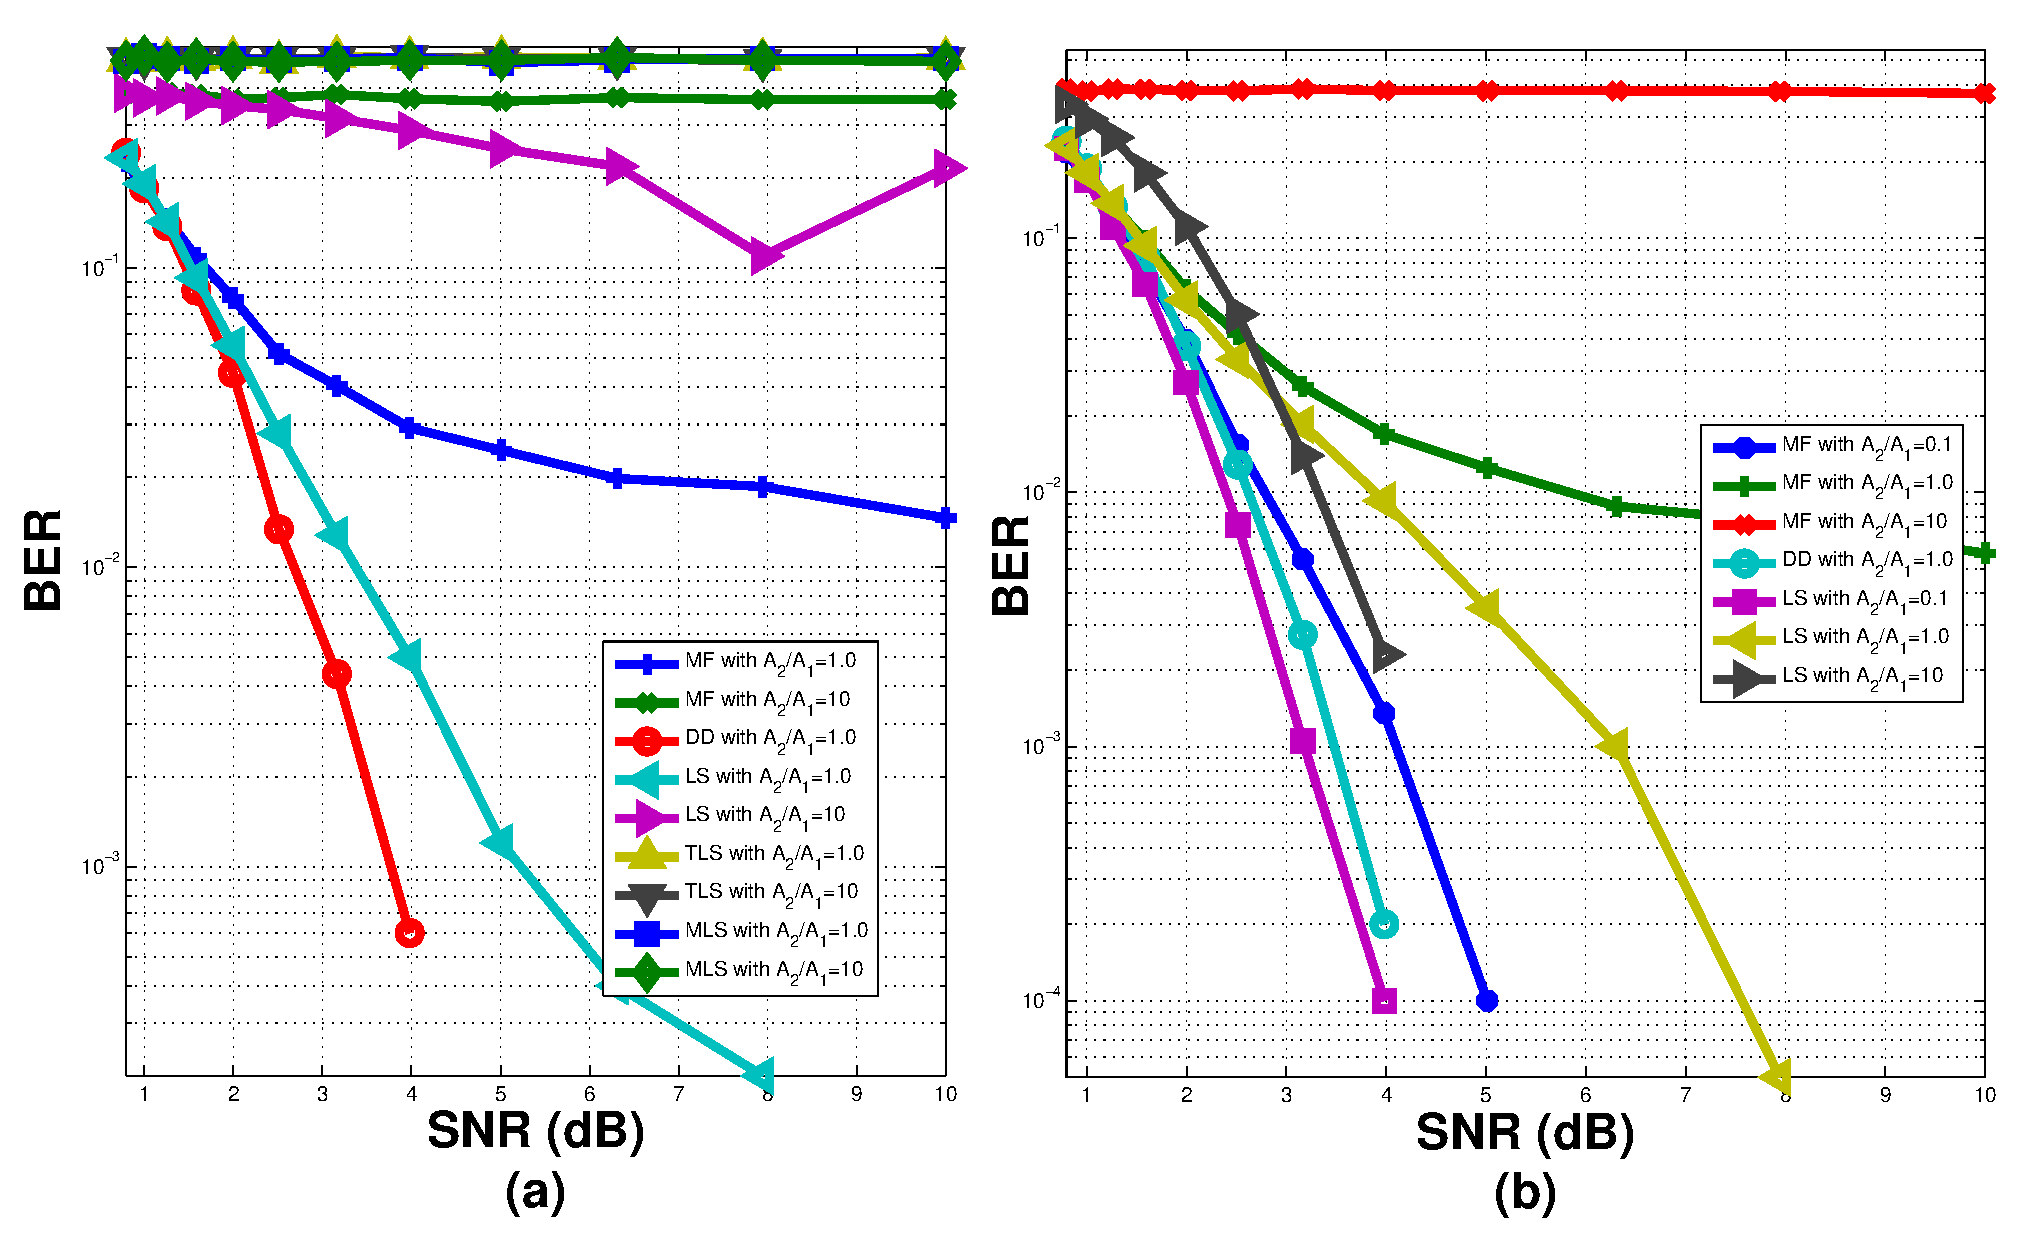
\includegraphics[width=3.0in]{BER_SNR_10_64.eps}
\caption{ (a) The performance of the proposed blind MUDs against
SNR, $M=12$. (b) The performance of the proposed blind LS
detector, $M=63$. } }\label{BER_SNR}
\end{figure}
\begin{figure} \center{
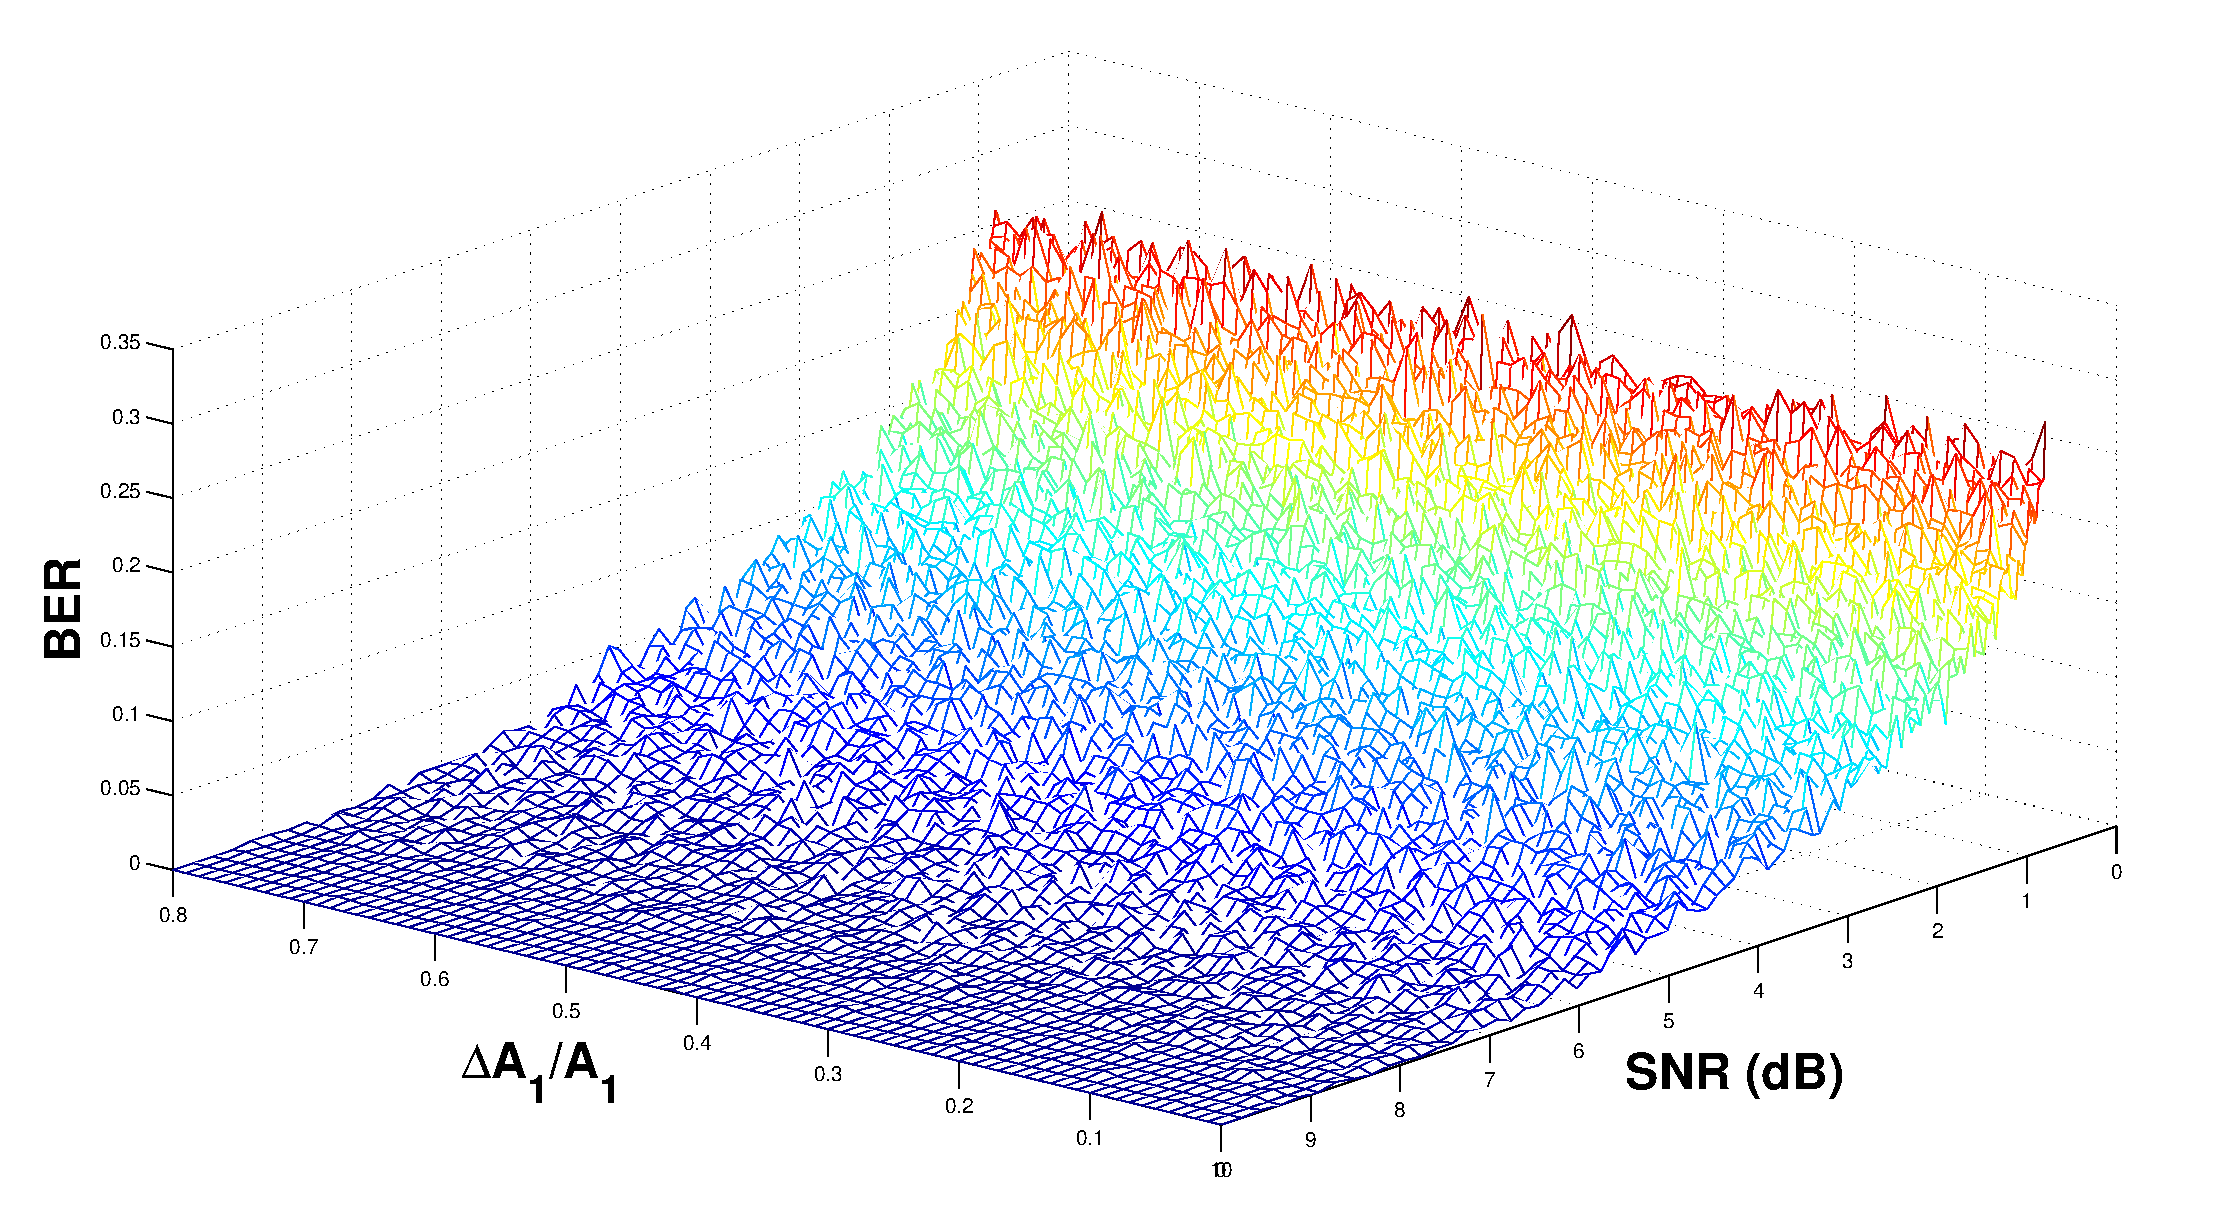
\includegraphics[width=2.50in]{BER_A_SNR_10_64_LSs.eps}
\caption{ The performance of the LS detector against amplitude
estimation error ${\Delta}{A_1}/A_1$ and SNR, $M=63$.}
}\label{BER_A_SNR}
\end{figure}
\begin{figure}
\center{
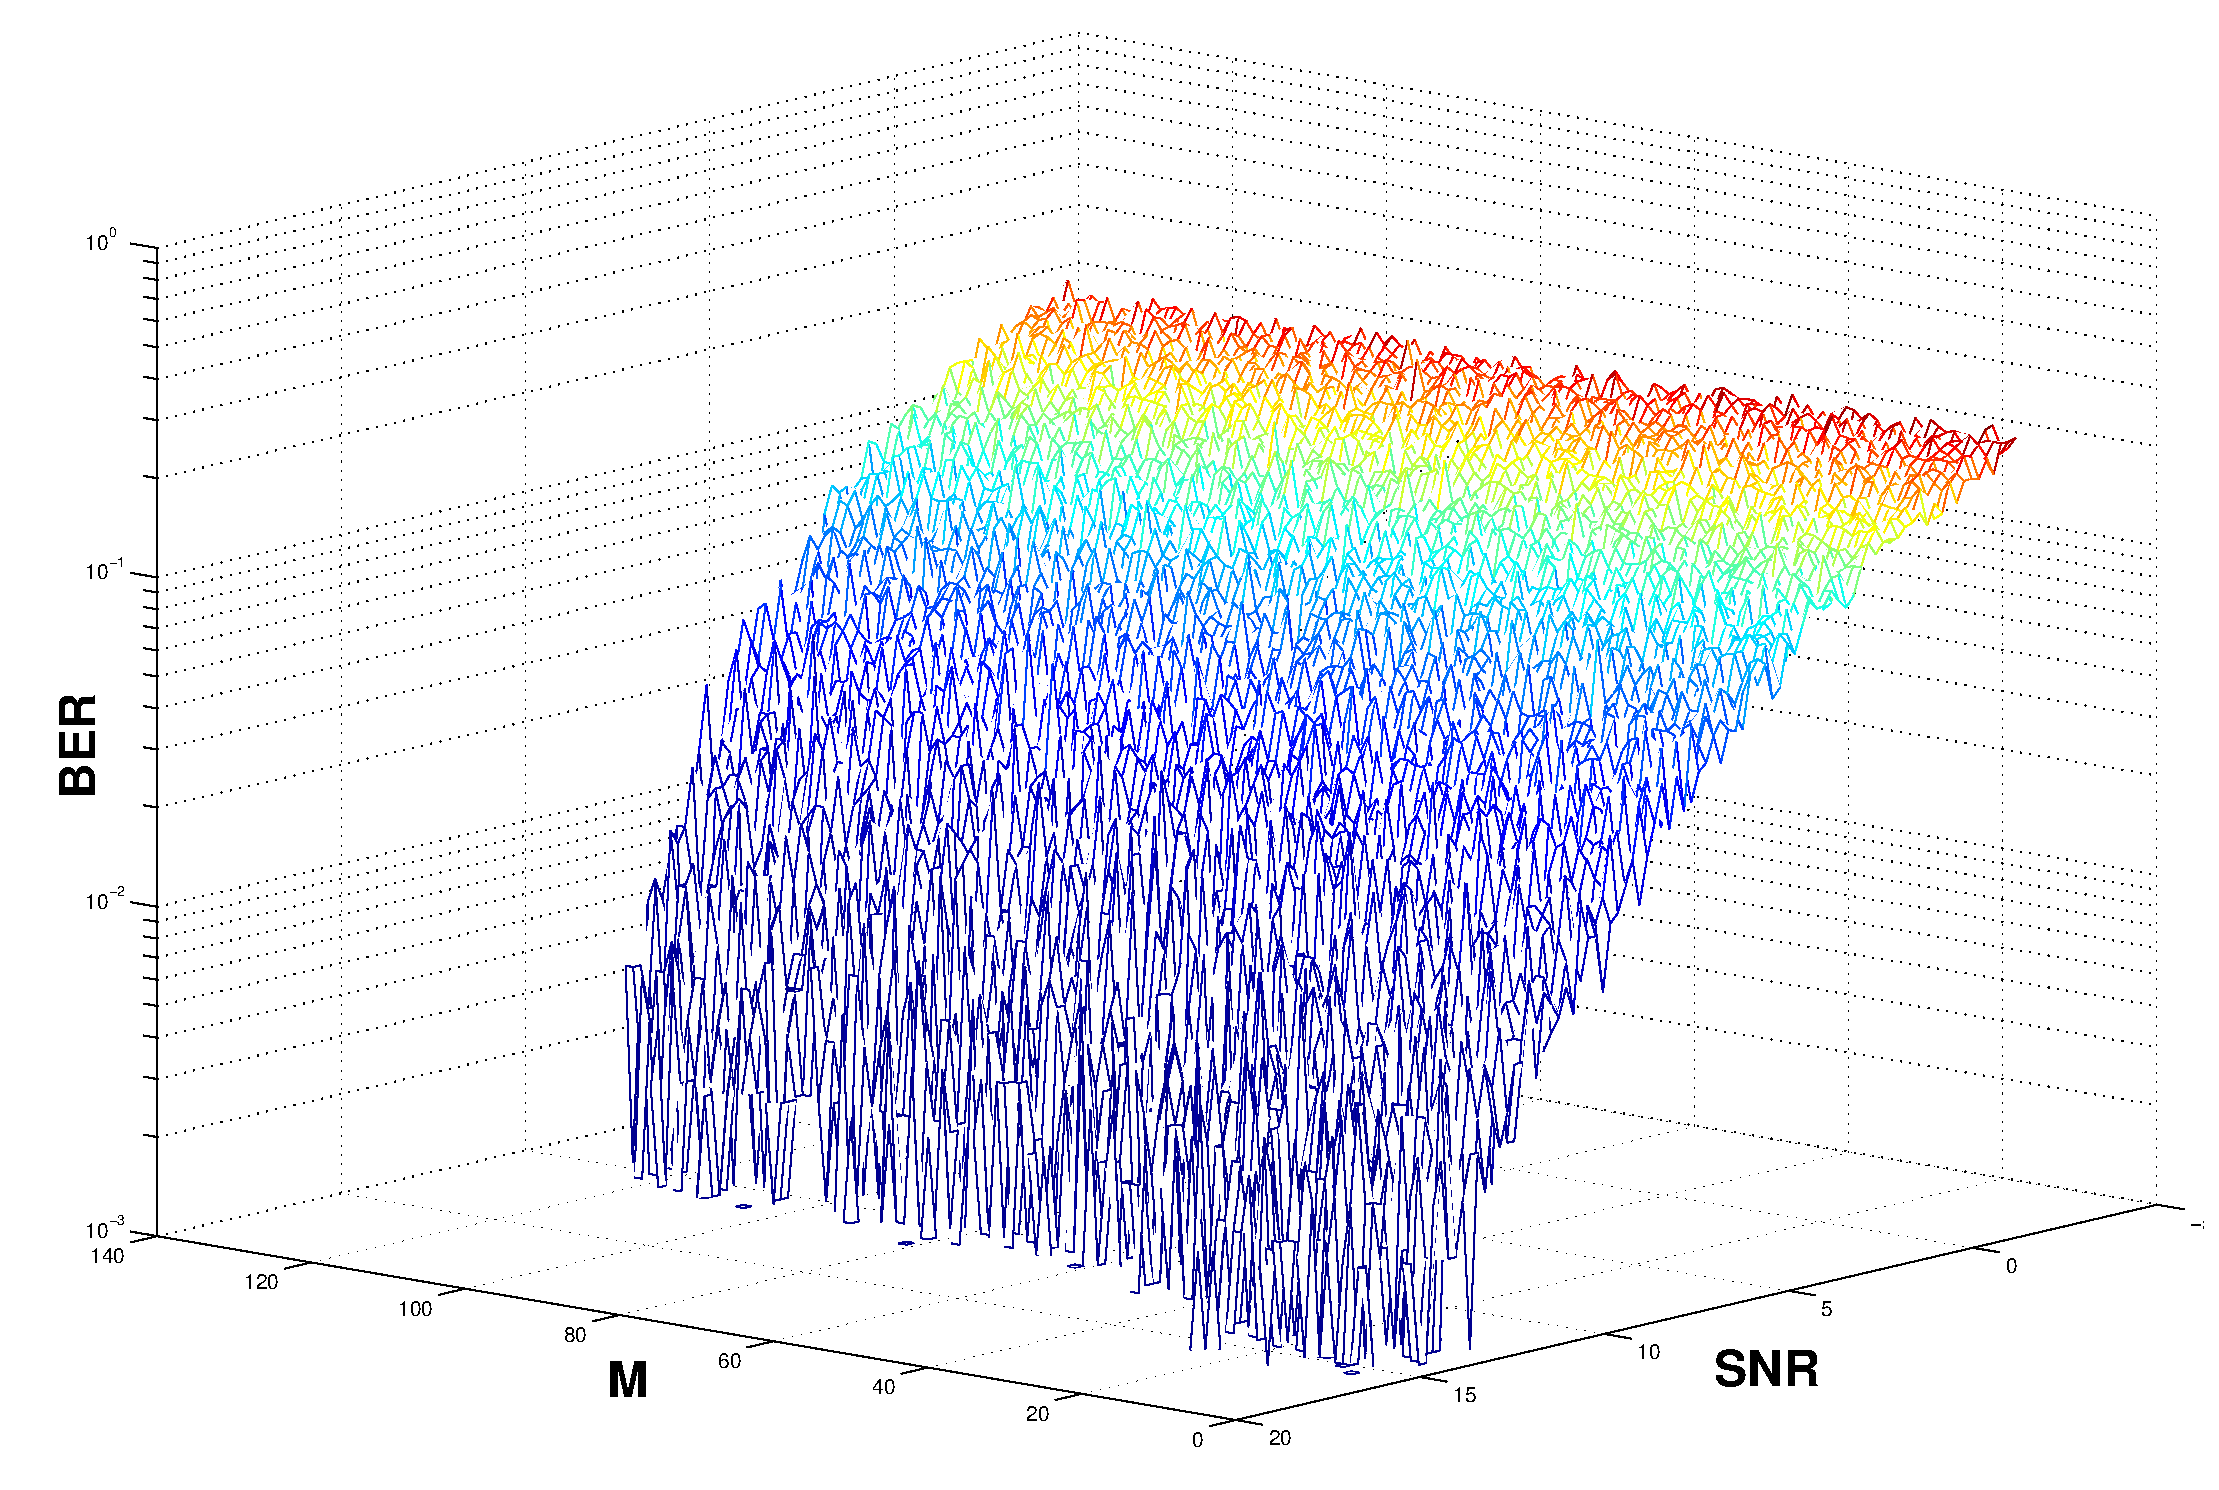
\includegraphics[width=2.50in]{BER_M_SNR_10_64_LSs.eps}
\caption{ The performance of the LS blind MUD against $M$ and
SNR.} }\label{BER_M_SNR}
\end{figure}

\section{Conclusions}
In this paper, we proposed an alternative approach for designing
blind multiuser detectors. The proposed blind multiuser detectors
are straightforward without any channel or spreading sequence
estimations employed by other existing blind detectors.

\small
\bibliographystyle{unsrt}
\bibliography{FastBDD}

\end{document}
